% DriftGate TMC — figure include snippets (IEEEtran). Vector PDFs; embedded fonts.
% F1,F2,F3,F4,F5 = double-column (figure*); F6 = single-column (figure).
% Widths chosen so inserted fonts stay >= 7 pt; do not rescale the same figure repeatedly.

\begin{figure*}[t]
  \centering
  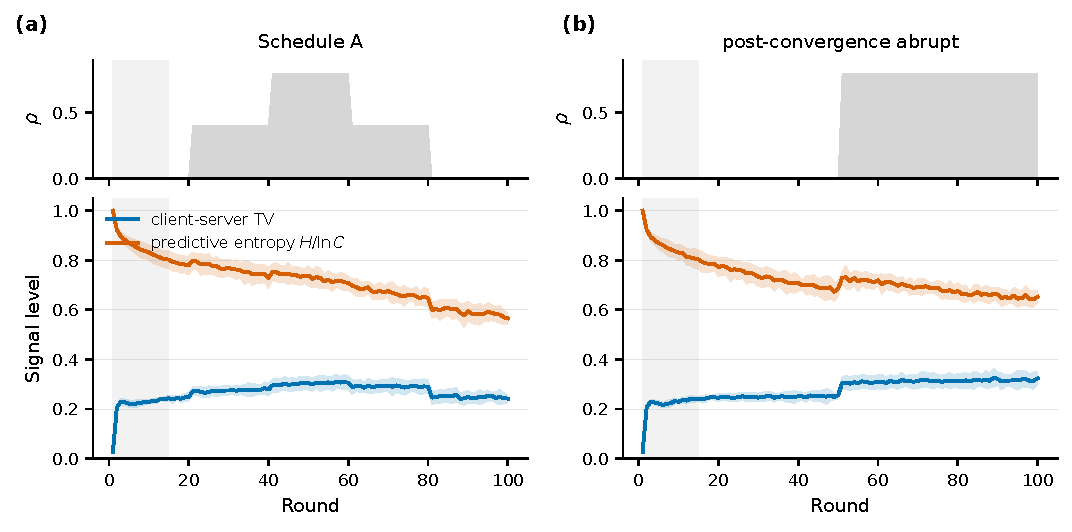
\includegraphics[width=\textwidth]{figures/fig01_signal_dynamics.pdf}
  \caption{Signal dynamics under continued training. Top: traffic-shift level $\rho$.
  Bottom: client--server TV (blue) and normalized predictive entropy $H/\ln C$ (orange),
  computed on the same fixed-weight model trajectory and the same requests (3 seeds; bands are
  seed SD). TV rises and falls with $\rho$, whereas entropy declines monotonically with
  convergence and even anti-correlates after the abrupt shift in (b). Warm-up rounds are shaded.}
  \label{fig:signal_dynamics}
\end{figure*}

\begin{figure*}[t]
  \centering
  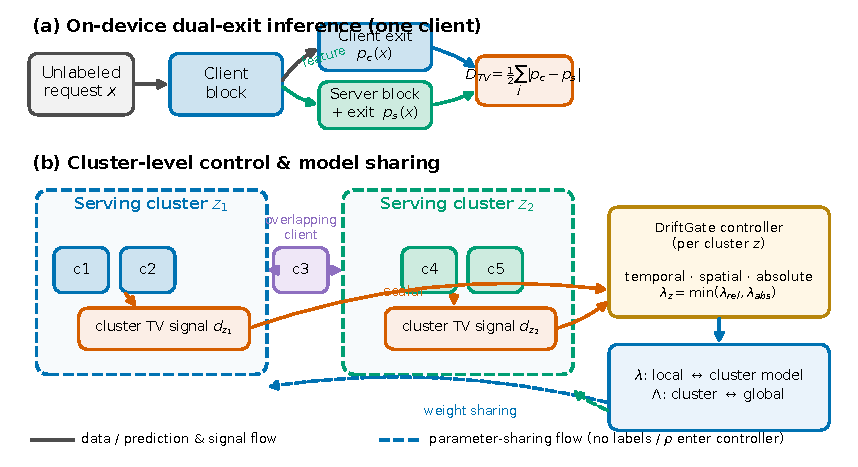
\includegraphics[width=0.82\textwidth]{figures/fig02_system_overview.pdf}
  \caption{DriftGate overview. (a) On-device dual exits: the client block feeds a client exit
  $p_c$ and, through the server block, a server exit $p_s$; their total variation $D_{TV}$ is the
  unlabeled drift signal. (b) Per-cluster control: client TV values are averaged into a cluster
  signal that the controller turns, via temporal/spatial/absolute views, into $\lambda$
  (local$\leftrightarrow$cluster) and $\Lambda$ (cluster$\leftrightarrow$global) mixing weights.
  Solid = data/prediction and signal flow, dashed = parameter sharing; no labels or $\rho$ enter
  the controller. Two clusters shown as an example.}
  \label{fig:overview}
\end{figure*}

\begin{figure*}[t]
  \centering
  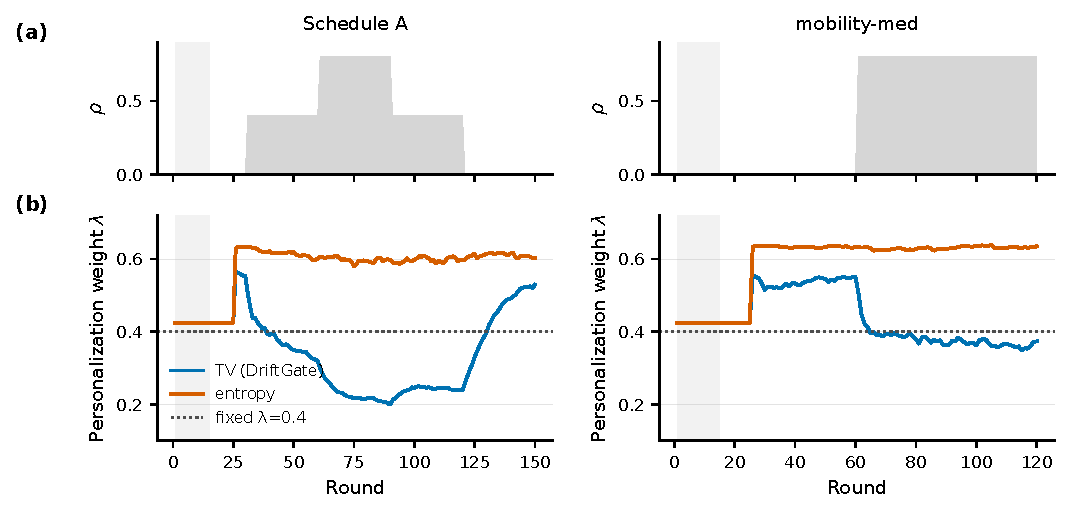
\includegraphics[width=\textwidth]{figures/fig03_lambda_adaptation.pdf}
  \caption{Traffic-shift to $\lambda$ adaptation under the disjoint protocol. Left: CIFAR-10
  Schedule~A (5 seeds); right: medium mobility (3 seeds). (a) $\rho$. (b) per-cluster-averaged
  $\lambda$ for TV and entropy with the fixed $\lambda{=}0.4$ reference. TV lowers $\lambda$ as
  $\rho$ rises and restores it afterwards, while entropy raises $\lambda$ regardless. Accuracy is
  reported in the results tables.}
  \label{fig:lambda_adaptation}
\end{figure*}

\begin{figure*}[t]
  \centering
  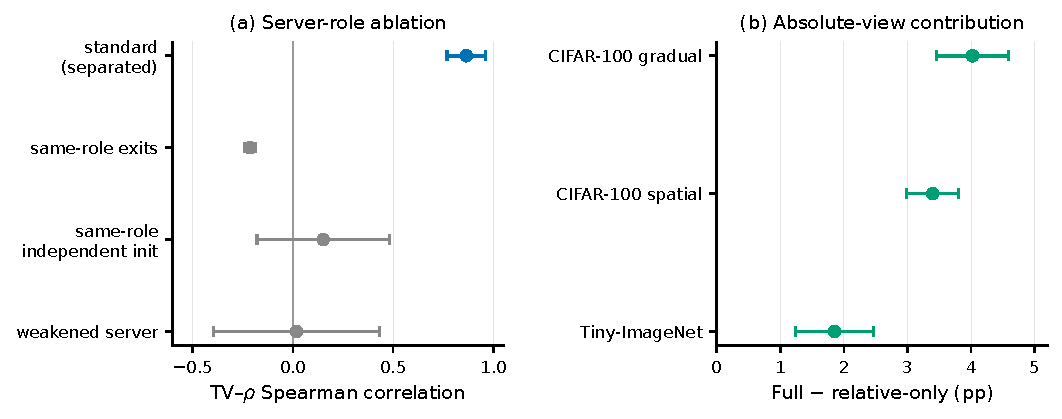
\includegraphics[width=\textwidth]{figures/fig04_mechanism_and_views.pdf}
  \caption{(a) Server-role ablation: TV--$\rho$ Spearman correlation across role perturbations
  (same-pool, 3 seeds; mean$\pm$SD). Separating the exits' roles is necessary for TV to track
  $\rho$. (b) Contribution of the absolute view: full controller minus a relative-only variant on
  transfer settings (development-version comparison, same-pool, 3 seeds; 95\% CI).}
  \label{fig:mechanism}
\end{figure*}

\begin{figure*}[t]
  \centering
  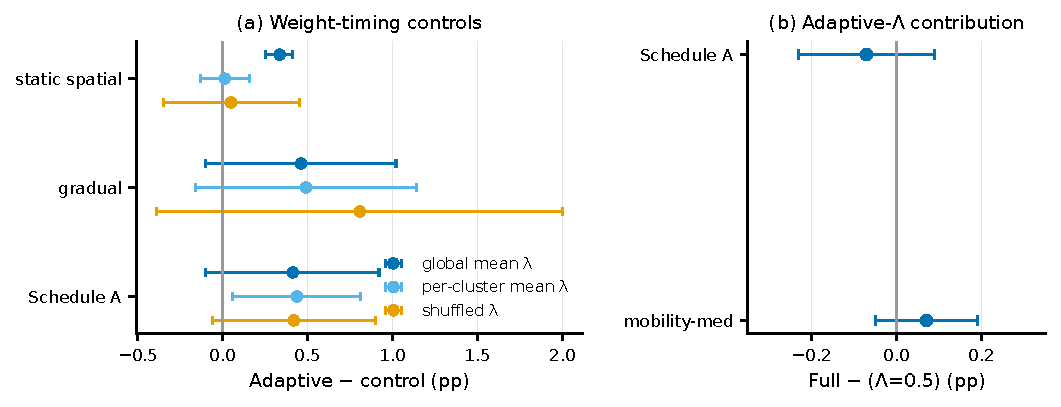
\includegraphics[width=\textwidth]{figures/fig05_timing_and_lambda.pdf}
  \caption{(a) Weight-timing controls: adaptive minus mean-matched and shuffled $\lambda$ policies
  (same-pool replay that retrains with the altered weight order; 3 seeds, 95\% CI). The
  static-spatial gain comes from good per-cluster means, not timing. (b) Adaptive-$\Lambda$
  contribution: full controller minus a $\Lambda{=}0.5$ variant (disjoint; 5/3 seeds). Both CIs
  include zero.}
  \label{fig:timing_lambda}
\end{figure*}

\begin{figure}[t]
  \centering
  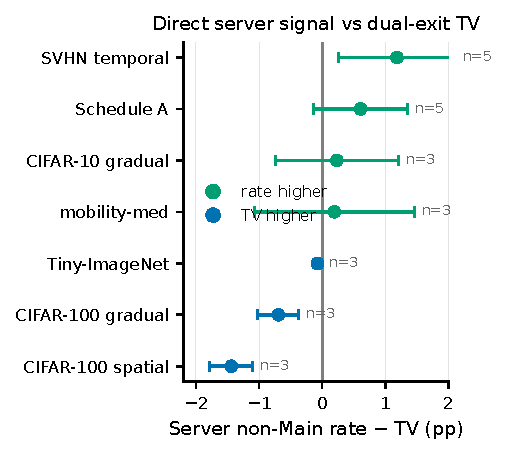
\includegraphics[width=\columnwidth]{figures/fig06_server_signal_comparison.pdf}
  \caption{Direct server-only signal vs dual-exit TV across seven settings (disjoint, paired;
  95\% CI). The server non-Main prediction rate matches or beats TV where the class count is small
  and drift is real (SVHN, CIFAR-10) but is weaker on many-class CIFAR-100. Green = rate higher,
  blue = TV higher.}
  \label{fig:server_signal}
\end{figure}
